Spending time and resources to model the dynamics of calcium channels is important as
Ca\(^{2+}\) is a highly veratile intracellular signal, involved into a considerable number
of cellular processes, among which spiking activity, plasticity, regulation of the contraction
at the muscular level, metabolism, and so on. Despite the same type of Ca\(^{2+}\) ions are
involved, the time scales of the mentioned processes are very different, as shown in the
picture below.
\begin{figure}[H]
    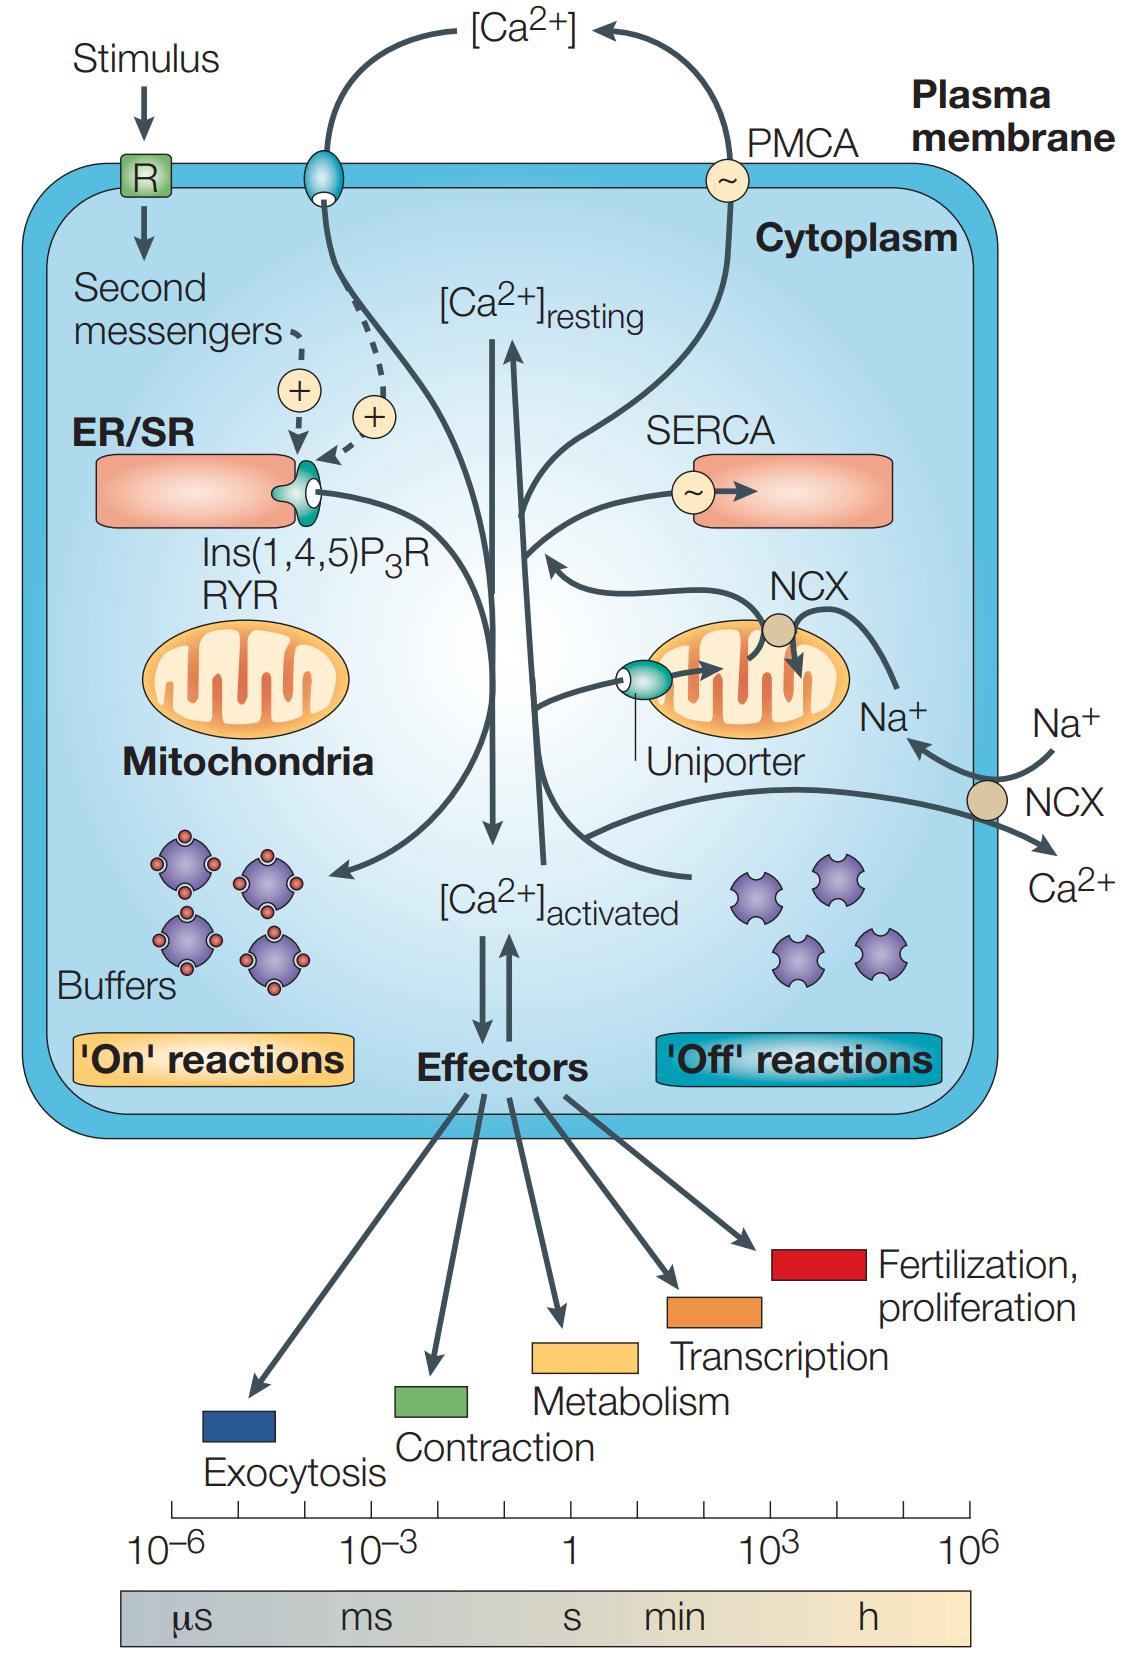
\includegraphics[scale=0.25]{11_1}
    \centering
\end{figure}
At the level of a single cell, a model of the intracellular calcium dynamics can be built.
It should involve four steps:
\begin{enumerate}
    \item The entry of Ca\(^{2+}\) into the cell via calcium channels.
    \item The diffusion of calcium throughout the cell, which cannot be neglected as the
          calcium concentration inside the cell is very low.
    \item The action of intracellular calcium binding proteins, said buffering.
    \item The efflux or uptake of Ca\(^{2+}\) ions via the action of membrane-bound pumps,
          which is usually disregarded.
\end{enumerate}
Note that if the cell is modelled as a sphere made of concentric shells or layers, with the
outer one containing punctual calcium sources representing the channels,
the change in intracellular calcium concentration due to the influx of Ca\(^{2+}\)
ions is formalized as:
\begin{equation*}
    \frac{\partial{[\text{Ca}^{2+}]_{in}}}{\partial{t}}=-\frac{1}{2\cdot{F}\cdot{V_{n}}}I_{Ca}
\end{equation*}
where \(V_{n}\) is the volume of the sphere and \(F\) is the Faraday constant.

\subsection{Calcium Diffusion Model}
Once the Ca\(^{2+}\) ions entered the cell from a punctual source, they start to diffuse
towards the center of the cell. To model such a phenomenon, also buffering is to be
considered, it is coupled to diffusion. The following profile represents the intracellular
calcium concentration \([\text{Ca}^{2+}]_in\) as a function of the distance \(x\) from the source.
\begin{figure}[H]
    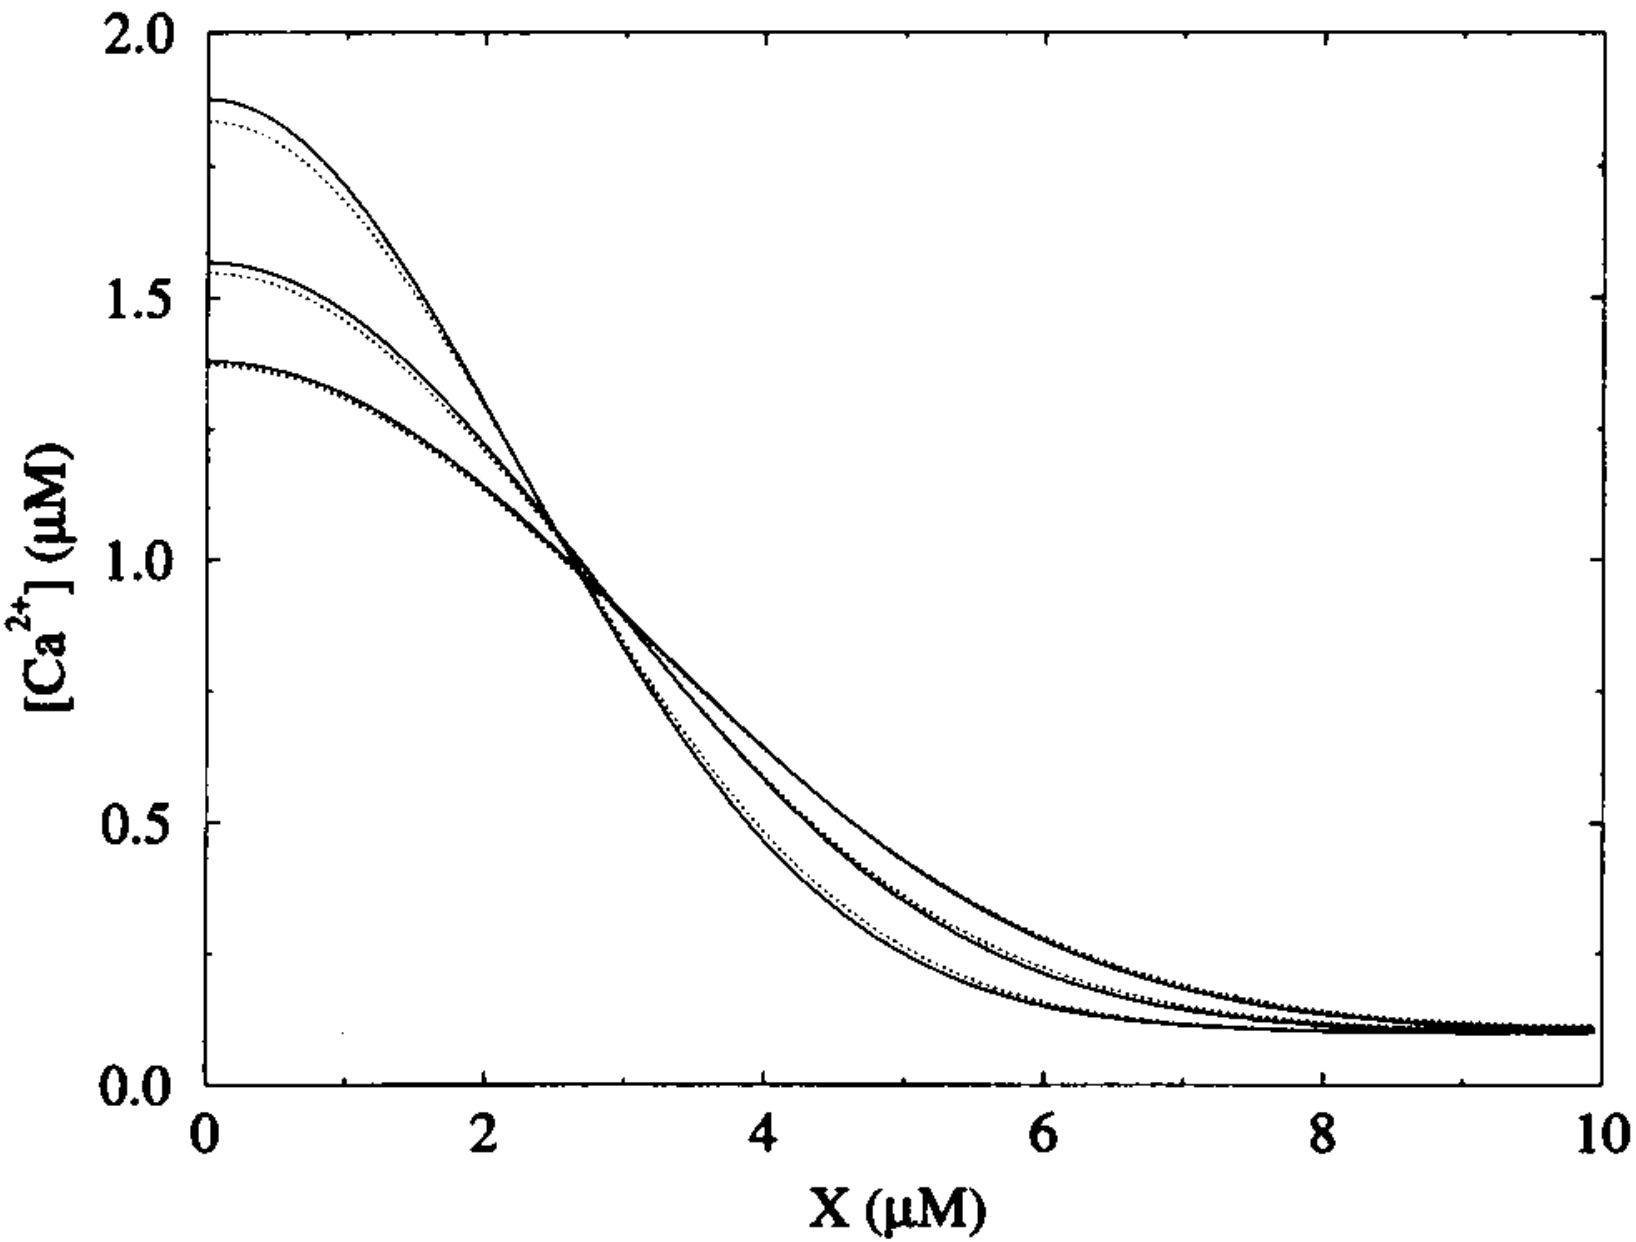
\includegraphics[scale=0.2]{11_2}
    \centering
\end{figure}
At this point, the buffered diffusion of Ca\(^{2+}\) can be mathematically described by a
system of reaction-diffusion equations with spherical symmetry. Note that B\(_{j}\) represents
the \(j\)-th species of buffer, while CaB\(_{j}\) is the calcium bound to the buffer.
\begin{equation*}
    \begin{cases}
        \frac{d\text{Ca}^{2+}}{dt}=-k^{+}_{j}[\text{Ca}^{2+}][\text{B}_{j}]+k^{-}_{j}[\text{CaB}_{j}]\equiv{R_{j}}
        \hspace{2cm}\text{Calcium kinetics}   \\
        \frac{d\text{B}_{j}}{dt}=-k^{+}_{j}[\text{Ca}^{2+}][\text{B}_{j}]+k^{-}_{j}[\text{CaB}_{j}]
        \hspace{3.42cm}\text{Buffer kinetics} \\
        \frac{d\text{CaB}_{j}}{dt}=-k^{-}_{j}[\text{CaB}_{j}]+k^{+}_{j}[\text{Ca}^{2+}][\text{B}_{j}]
        \hspace{3.075cm}\text{Calcium + Buffer kinetics}
    \end{cases}
\end{equation*}
By recalling the 2nd Fick Law
\begin{equation*}
    \frac{\partial{c_{i}}}{\partial{t}}=D_{i}\nabla^{2}c_{i}
\end{equation*}
where \(c_{i}\) is the concentration of the \(i\)-th species, the previous system can be
rewritten as:
\begin{equation*}
    \begin{cases}
        \frac{d\text{Ca}^{2+}}{dt}=D_{\text{Ca}}\nabla^{2}[\text{Ca}^{2+}]+\sum_{j}R_{j} \\
        \frac{d\text{B}_{j}}{dt}=D_{\text{B}_{j}}\nabla^{2}[\text{B}_{j}]+\sum_{j}R_{j}  \\
        \frac{d\text{CaB}_{j}}{dt}=D_{\text{CaB}_{j}}\nabla^{2}[\text{CaB}_{j}]-\sum_{j}R_{j}
    \end{cases}
\end{equation*}
Note that \(D_{\text{Ca}}\), \(D_{\text{B}_{j}}\), and \(D_{\text{CaB}_{j}}\) are the
diffusion coefficients.\\
To further simplify the model, it is assumed that the buffer does not diffuse
\(\Rightarrow{D_{\text{B}_{j}}=D_{\text{CaB}_{j}}=0}\). Thus, to sum up,
other three hypothesis are considered:
\begin{enumerate}
    \item Calcium enters via punctual sources and its concentration at steady-state is fixed.
    \item There are no sources for the buffer, thus it has a fixed concentration
          \([\text{B}_{j}]_{T}=[\text{B}_{j}]+[\text{CaB}_{j}]\).
    \item Far from the sources, calcium and buffer are in equilibrium.
\end{enumerate}
\paragraph{Evaluation of \([\text{B}_{j}]_{\infty}\)} In steady-state conditions
\(\frac{d\text{B}_{j}}{dt}=0\), therefore:
\begin{gather*}
    -k^{+}_{j}[\text{Ca}^{2+}]_{\infty}[\text{B}_{j}]_{\infty}+k^{-}_{j}[\text{CaB}_{j}]_{\infty}=0\\
    k^{+}_{j}[\text{Ca}^{2+}]_{\infty}[\text{B}_{j}]_{\infty}=k^{-}_{j}[\text{CaB}_{j}]_{\infty}\\
    k^{+}_{j}[\text{Ca}^{2+}]_{\infty}[\text{B}_{j}]_{\infty}=k^{-}_{j}\bigl([\text{B}_{j}]_{T}-[\text{B}_{j}]_{\infty}\bigr)
    \bigl(k^{+}_{j}[\text{Ca}^{2+}]_{\infty}+k^{-}_{j}\bigr)[\text{B}_{j}]_{\infty}=k^{-}_{j}[\text{B}_{j}]_{T}\\
    \Rightarrow
    [\text{B}_{j}]_{\infty}
    =\frac{k^{-}_{j}[\text{B}_{j}]_{T}}{k^{+}_{j}[\text{Ca}^{2+}]_{\infty}+k^{-}_{j}}
    =\frac{\frac{k^{-}_{j}}{k^{+}_{j}}[\text{B}_{j}]_{T}}{[\text{Ca}^{2+}]_{\infty}+\frac{k^{-}_{j}}{k^{+}_{j}}}
    =\frac{K_{j}[\text{B}_{j}]_{T}}{[\text{Ca}^{2+}]_{\infty}+K_{j}}
\end{gather*}
where \(K_{j}=\frac{k^{-}_{j}}{k^{+}_{j}}\) is the dissociation constant for buffer \(j\).\\
Similarly, also the steady-state value \([\text{CaB}_{j}]_{\infty}\) can be computed.\\
\par
To further simplify the system of equation let's now consider the following assumptions:
\begin{enumerate}
    \item The diffusion constant of each mobile buffer is not affected by the Ca\(^{2+}\) binding,
          thus \(D_{\text{B}_{j}}=D_{\text{CaB}_{j}}\).
    \item \([\text{B}_{j}]_{T}\) is uniform along the whole temporal evolution.
\end{enumerate}
Hence,
\begin{equation*}
    \frac{d\text{CaB}_{j}}{dt}=D_{\text{CaB}_{j}}\nabla^{2}[\text{CaB}_{j}]-\sum_{j}R_{j}
\end{equation*}
can be neglected from the system and
\begin{equation*}
    R_{j}=-k^{+}_{j}[\text{Ca}^{2+}][\text{B}_{j}]+k^{-}_{j}\bigl([\text{B}_{j}]_{T}-[\text{B}_{j}]\bigr)
\end{equation*}
Moreover, the following hypothesis can be exploited to make the system easier:
\begin{enumerate}
    \item The buffer does not diffuse \(\Rightarrow{D_{\text{B}_{j}}=D_{\text{CaB}_{j}}=0}\).
    \item There is only one buffer species, thus \([\text{B}_{j}]=[\text{B}]\).
\end{enumerate}
As a consequence, the following system at steady-state is obtained:
\begin{equation*}
    \begin{cases}
        0=D_{\text{Ca}}\nabla^{2}[\text{Ca}^{2+}]-k^{+}[\text{Ca}^{2+}][\text{B}]+k^{-}\bigl([\text{B}]_{T}-[\text{B}]\bigr) \\
        0=D_{\text{B}}\nabla^{2}[\text{B}]-k^{+}[\text{Ca}^{2+}][\text{B}]+k^{-}\bigl([\text{B}]_{T}-[\text{B}]\bigr)
    \end{cases}
\end{equation*}
Now, the system can be finally reduced with a further assumptions, however there are two possible strategies:
\begin{itemize}
    \item Excess Buffer Approximation (EBA)
    \item Rapid Buffer Approximation (RBA)
\end{itemize}
\subsubsection{Excess Buffer Approximation}
Here it is assumed that the mobile buffer is present in excess and cannot be saturated, thus
\([\text{B}]=[\text{B}]_{\infty}\).
Hence, the system of differential equations at steady-state becomes the following:
\begin{equation*}
    \begin{cases}
        0=D_{\text{Ca}}\nabla^{2}[\text{Ca}^{2+}]-k^{+}[\text{Ca}^{2+}][\text{B}]_{\infty}+k^{-}\bigl([\text{B}]_{T}-[\text{B}]_{\infty}\bigr) \\
        0=D_{\text{B}}\cancelto{0}{\nabla^{2}[\text{B}]_{\infty}}-k^{+}[\text{Ca}^{2+}]_{\infty}[\text{B}]_{\infty}+k^{-}\bigl([\text{B}]_{T}-[\text{B}]_{\infty}\bigr)
    \end{cases}
\end{equation*}
Leading to the following single equation:
\begin{gather*}
    D_{\text{Ca}}\nabla^{2}[\text{Ca}^{2+}]-k^{+}[\text{Ca}^{2+}][\text{B}]_{\infty}+\cancel{k^{-}\bigl([\text{B}]_{T}-[\text{B}]_{\infty}\bigr)}
    =-k^{+}[\text{Ca}^{2+}]_{\infty}[\text{B}]_{\infty}+\cancel{k^{-}\bigl([\text{B}]_{T}-[\text{B}]_{\infty}\bigr)}\\
    \Rightarrow
    0=D_{\text{Ca}}\nabla^{2}[\text{Ca}^{2+}]-k^{+}[\text{B}]_{\infty}\Bigl([\text{Ca}^{2+}]-[\text{Ca}^{2+}]_{\infty}\Bigr)
\end{gather*}
This one is a linear equation in \([\text{Ca}^{2+}]\) and can be solved as follows:
\begin{equation*}
    [\text{Ca}^{2+}]=\frac{\sigma}{2\pi{D_{C}r}}\cdot{e^{-\frac{r}{\lambda}}}+[\text{Ca}^{2+}]_{\infty}
\end{equation*}
exhibiting an exponential decay, with \(\lambda=\sqrt{\frac{D_{C}}{k^{+}[\text{B}]_{\infty}}}\) being
the characteristic length constant and \(r\) being the radius of the sphere.\\
In the following plots it can be observed how the calcium concentration decreases as the distance
\(r\) increases, due to diffusion.
\begin{figure}[H]
    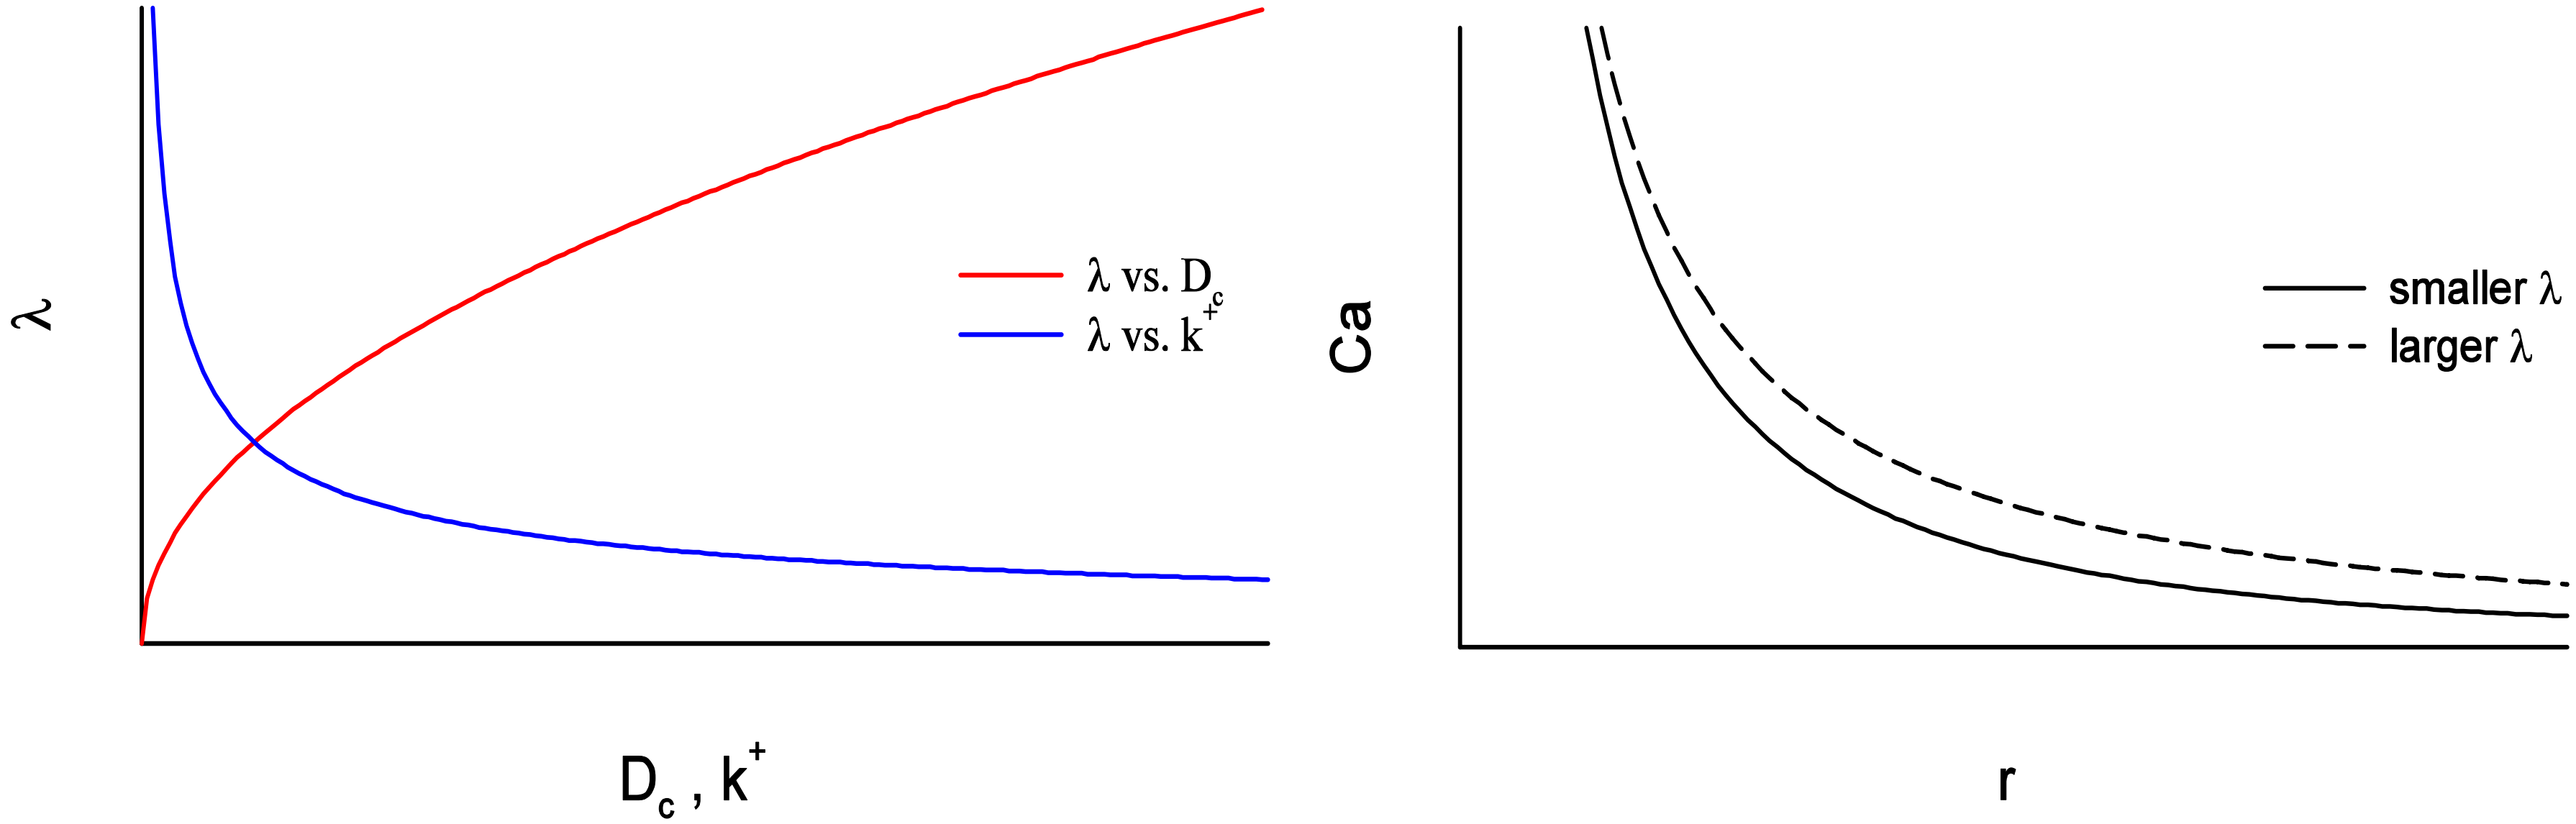
\includegraphics[scale=0.2]{11_3}
    \centering
\end{figure}
EBA is appropriate when the saturability of the mobile buffer is negligible.
\subsubsection{Rapid Buffer Approximation}
This approximation assumes the Ca\(^{2+}\) binding to the buffer to be considerably faster than
the calcium diffusion and this leads to local equilibrium: at every point in space the Ca\(^{2+}\)
and buffer are in equilibrium. Also in this case the system can be rewritten with a single equation:
\begin{equation*}
    \frac{dw}{dt}=\Bigl[D_{c}\beta+D_{b}(1-\beta)\Bigr]\nabla^{2}w
\end{equation*}
Note that \(\beta\) is a function of the total mobile buffer concentration and Ca\(^{2+}\).\\
RBA is appropriate when there is significant saturability of the mobile buffer and when the buffer
kinetics are fast with respect to the diffusion of Ca\(^{2+}\) ions.

\subsection{Considerations for Realistic Models}
A more realistic scenario requires to have multple calcium channels, each one with different dynamics.
Punctual sources spread throughout the spheric model of the membrane.\\
Another element crucial in realistic model is a mechanism to remove the intracellular calcium ions and
two choices are available:
\begin{itemize}
    \item \textbf{Exchangers}: the Na\(^{+}\)-Ca\(^{2+}\) exchangers are systems exploiting the sodium
          gradient to remove calcium ina \(3:1\) ratio.
    \item \textbf{Pumps}: the Ca-ATPase pumps are another alternative to model the removal of calcium ions.
\end{itemize}